\documentclass[]{article}
\usepackage{amsmath}
\usepackage{amsfonts}
\usepackage{amssymb}
\usepackage{tikz}
\usepackage{graphicx}
\usepackage{listings}

\definecolor{dkgreen}{rgb}{0,0.6,0}
\definecolor{gray}{rgb}{0.5,0.5,0.5}

\lstset{
  language=Python,
  breaklines=true,
  showstringspaces=false,
  frame=single,
  aboveskip=3mm,
  belowskip=3mm,
  columns=flexible,
  basicstyle={\small\ttfamily},
  numbers=none,
  numberstyle=\tiny\color{gray},
  keywordstyle=\color{blue},
  commentstyle=\color{gray},
  stringstyle=\color{dkgreen},
  breakatwhitespace=true,
  tabsize=3
}

\title{CAGD - Homework 6}
\author{Josefine St{\aa}l \& Erik Ackzell}

\begin{document}

\maketitle
\section*{Task 1}
In this task we plot a 3D Bretzel using B-splines. The code can be seen in Appendix I and the figure can be seen in the two figures below, from different angles.\\

\begin{figure}[h!]
	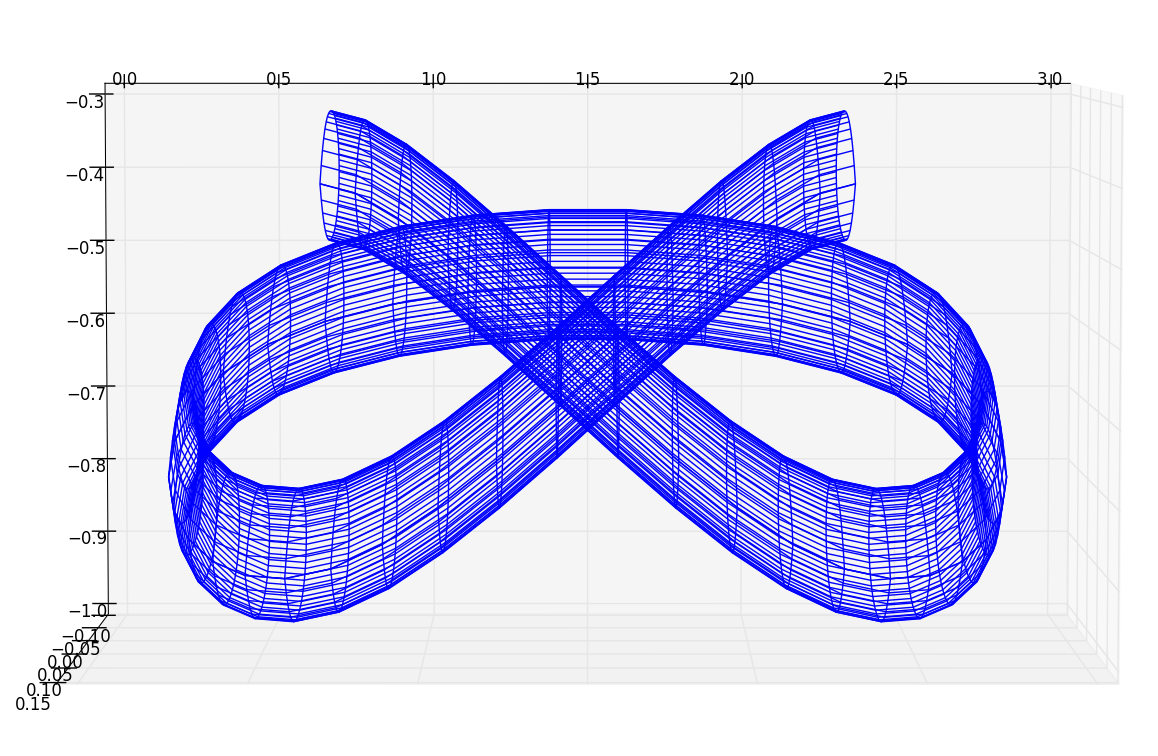
\includegraphics[scale=0.3]{bretzel3d2}
\end{figure}
\begin{figure}[h!]
	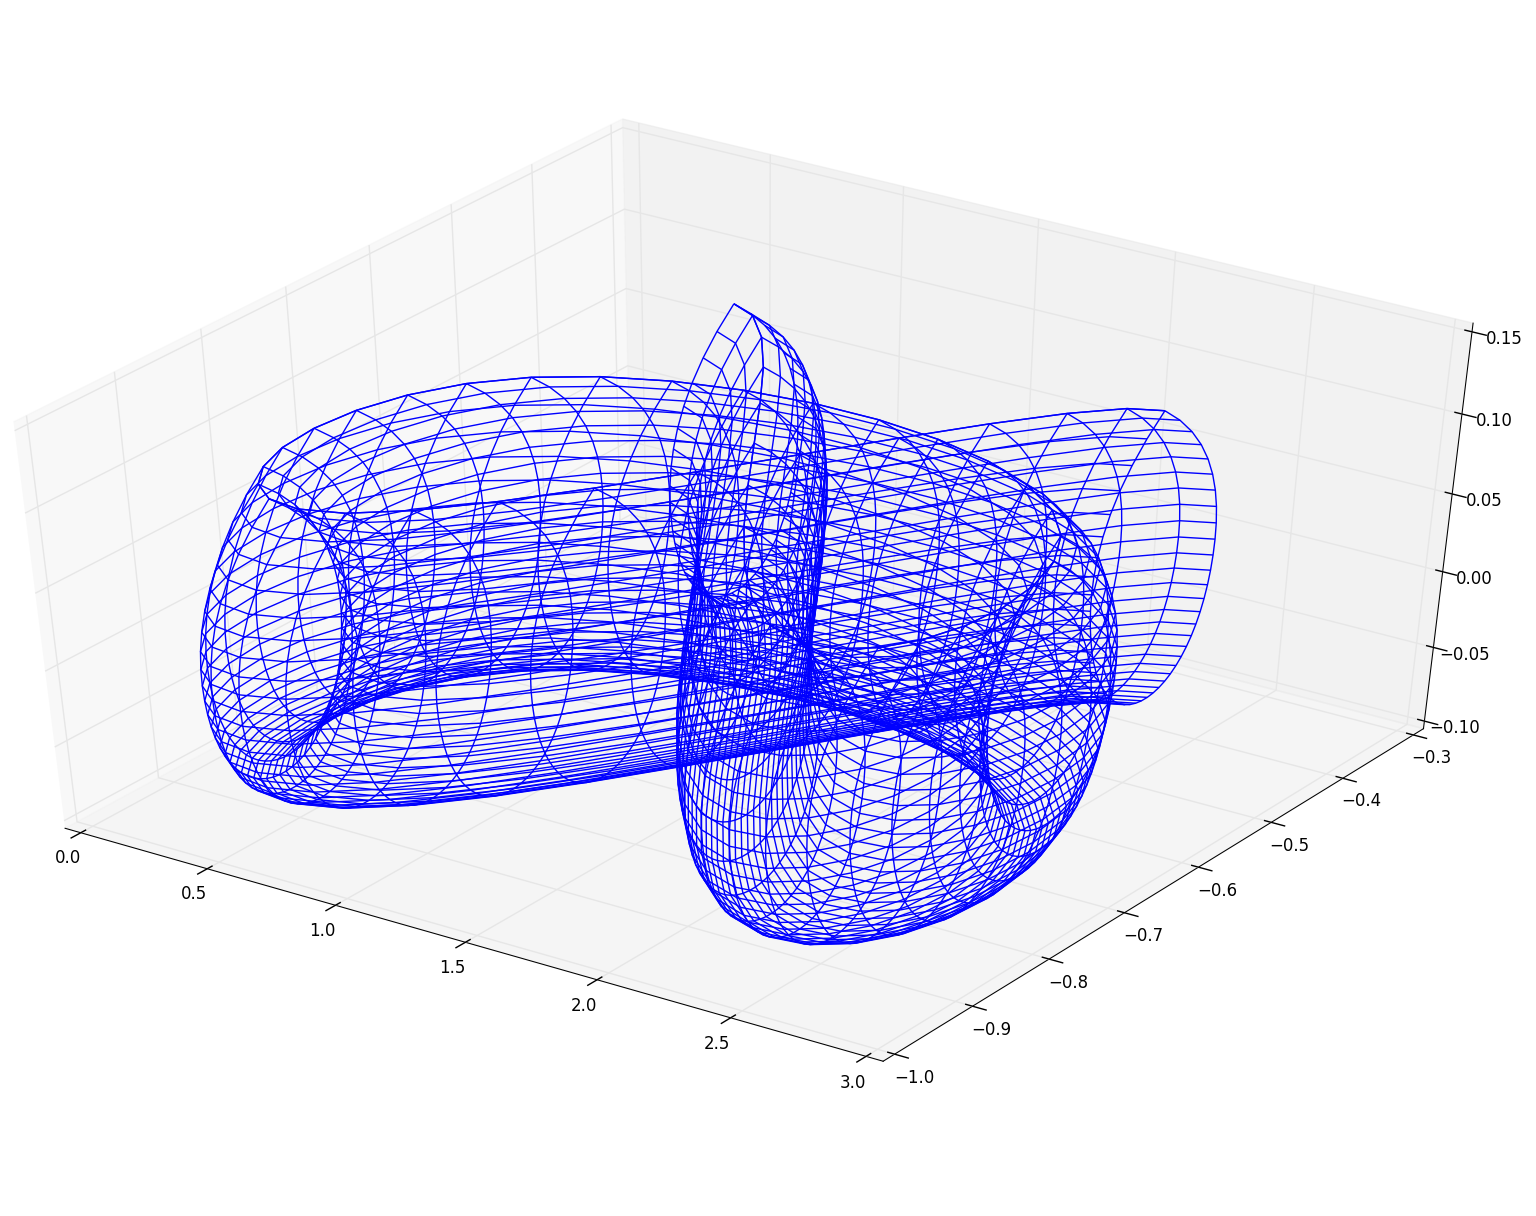
\includegraphics[scale=0.3]{bretzel3d}
\end{figure}

\newpage
\section*{Appendix I}
\lstinputlisting[firstline=7]{task1.py}

\end{document}
